\begin{frame}[t,plain]
\titlepage
\end{frame}



\begin{frame}[t]{Motivación del proyecto}


\begin{center}
\underline{Mucho} es el tiempo desperdiciado en el laboratorio armado y desarmando el setup, alineando cada etapa.
\end{center}

\begin{minipage}{0.5\textwidth}
Caracterizar haces de fuentes conlleva
\begin{itemize}
\item Perfil espacial. Divergencia
\item Perfil espectral y temporal
\item Polarización
\end{itemize}

\end{minipage}
%
\begin{minipage}{0.45\textwidth}
\begin{figure}[H]
\centering
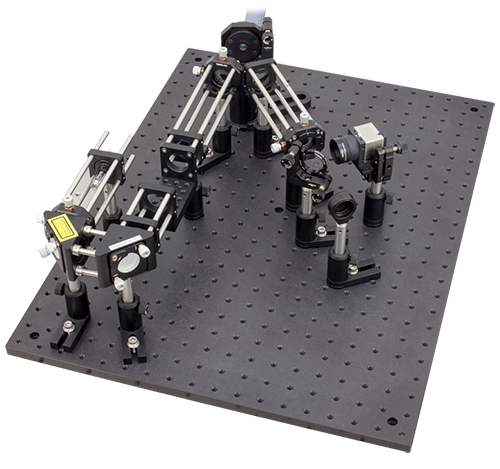
\includegraphics[width=\textwidth]{fig/optic_setup}
%\caption{}
\label{fig:optic_setup}
\end{figure}
\end{minipage}

\end{frame}


\begin{frame}[fragile]{Concepto del perfilador}
\begin{onlyenv}<1>
    \begin{columns}
        \begin{column}{0.5\textwidth}
        
            \begin{itemize}
                \item Determinar el perfil especial del haz en un plano
                \item Al desplazarse permite determina la divergencia del haz.
                \item Perfiladores con cámaras CCD. Sensores muy caros
                \item Perfiladores integradores. Complejidad mecánica
            \end{itemize}
        \end{column}
        
        \begin{column}{0.5\textwidth}
            \begin{figure}[H]
            \centering
            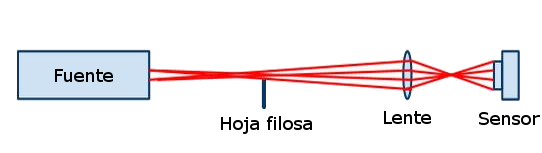
\includegraphics[width=\textwidth]{fig/perfilador/esquema_basico}
            \label{fig:perfilador/esquema_basico}
            \end{figure}
        \end{column}
    \end{columns}
\end{onlyenv}

\begin{onlyenv}<2>
\centering
Para haces gaussianos (\underline{la mayoría}), el perfil de intensidades, es decir la integral del perfil, es la función error

\begin{figure}
\centering
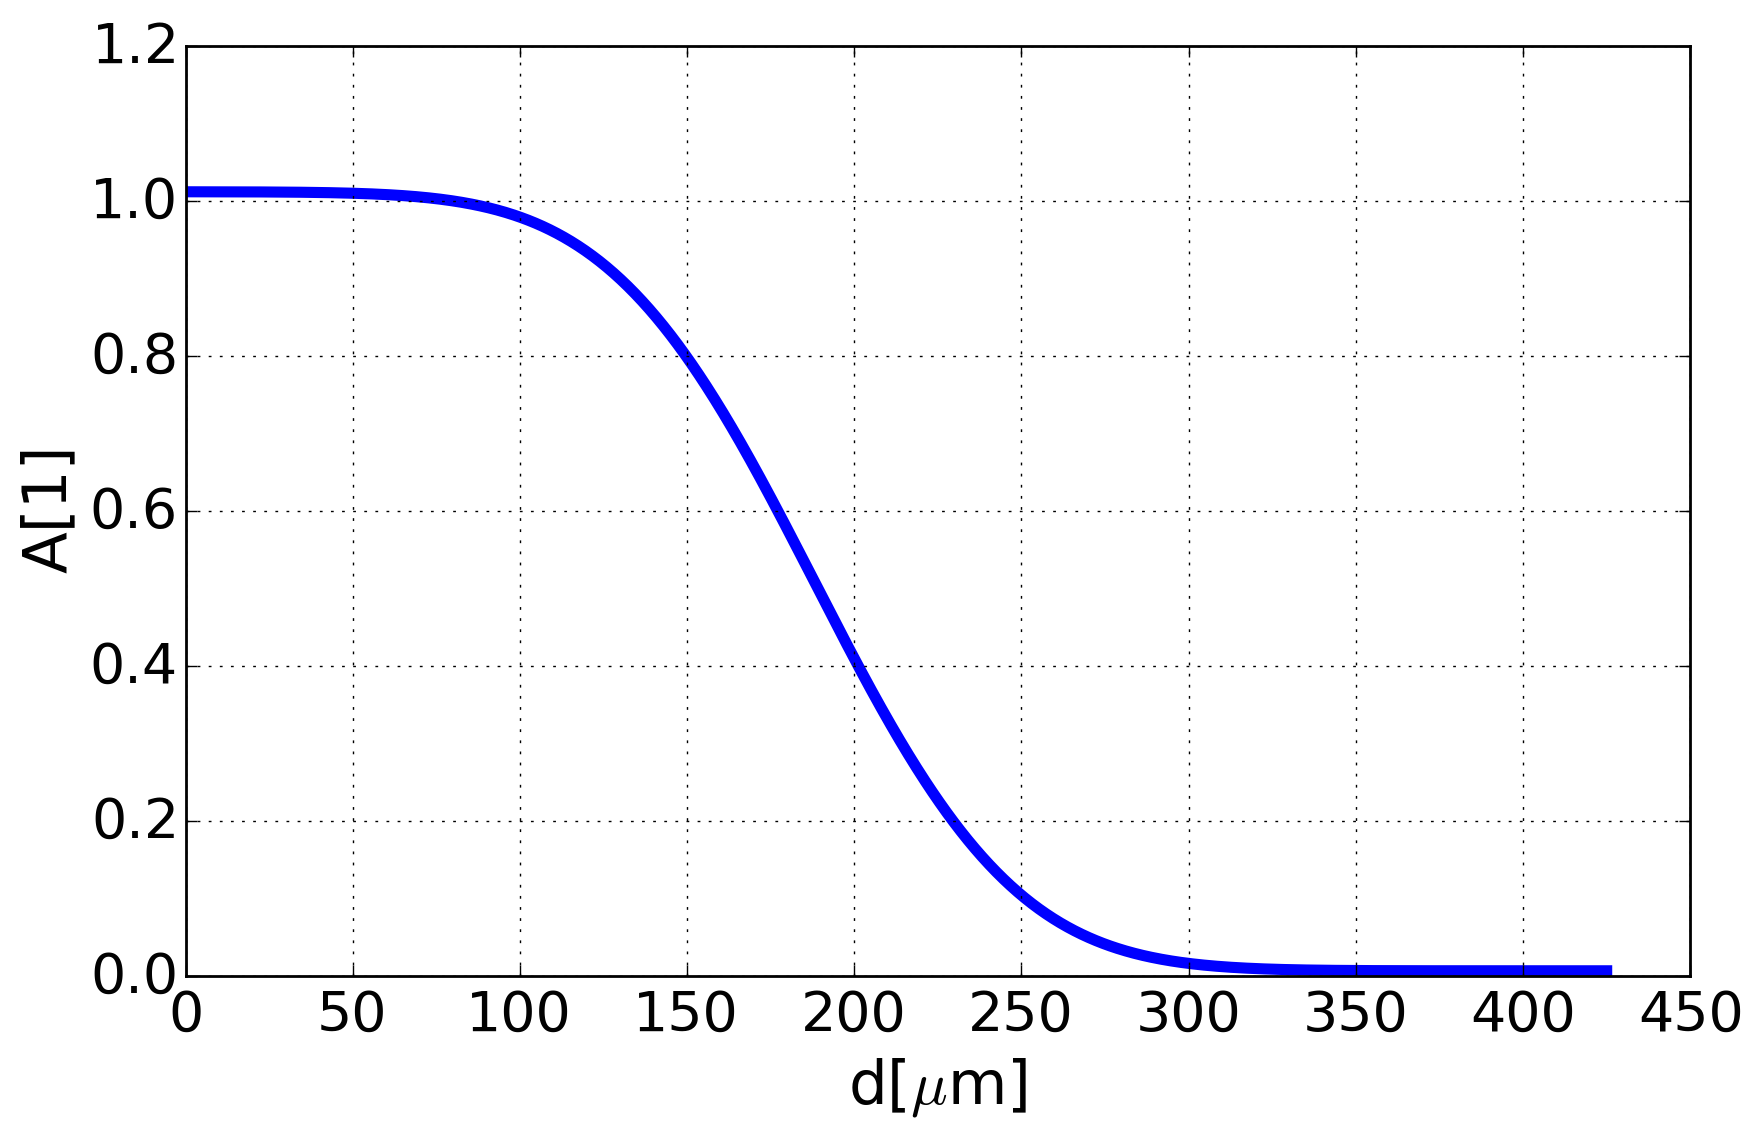
\includegraphics[width=0.8\textwidth]{fig/perfilador/err_function.png}
\label{fig:perfilador/err_function}
\end{figure}

\end{onlyenv}

\end{frame}

\begin{frame}[fragile]{Concepto del polarizador}

\begin{figure}[H]
\centering
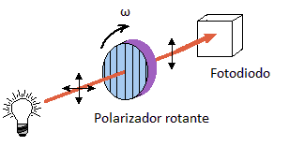
\includegraphics[width=0.4\textwidth]{fig/polarimetro/esquema}
%\caption{}
\label{fig:polarimetro}
\end{figure}
\begin{itemize}
\item Permite determinar eje mayor y eje menor de polarización eliptica. 
\item Permite identificar polarización circular.
\item Con un sistema de engranajes y con microstepping se puede tener una precisión importante. Con los motores usados, minimo 1.8$^\circ$.
\end{itemize}


\end{frame}

\section{Reseña Labo 6}

\begin{frame}{Perfilador en Laboratorio 6}

    
    \begin{onlyenv}<1>
        Resumen de especificaciones del perfilador construido
        \begin{itemize}
            \item Permite perfilar haces hasta 10$\,$cm de diametro 
            \item Utiliza un fotodiodo de amplio espectro, que permite medir haces grandes.
            \item Adaptado para los diferentes setups del laboratorio.
            \item Actualizar un perfil por segundo, debido a problemas mecánicos y de transmisión. No puede ser en tiempo real
            \item Diferencias en cada transición del perfilador. Produce un error del 50\%.
        \end{itemize}
    \end{onlyenv}

    \begin{onlyenv}<2>
        Piezas mecánicas del perfilador
        \begin{columns}[c]
            \begin{column}{.5\textwidth}
                \begin{itemize}
                \item Diseño autoportante.
                \item Tambor de perfilación permite medir en sistema Cage de Thorlabs. Permite medir divergencias importantes
                \item Tambor impreso en 3D.
                \item Motor paso a paso NEMA 17. 200 pasos por vuelta. Máximo 15rps. 
                \end{itemize}
            \end{column}
            %
            \begin{column}{0.5\textwidth}
                \begin{figure}
                \centering
                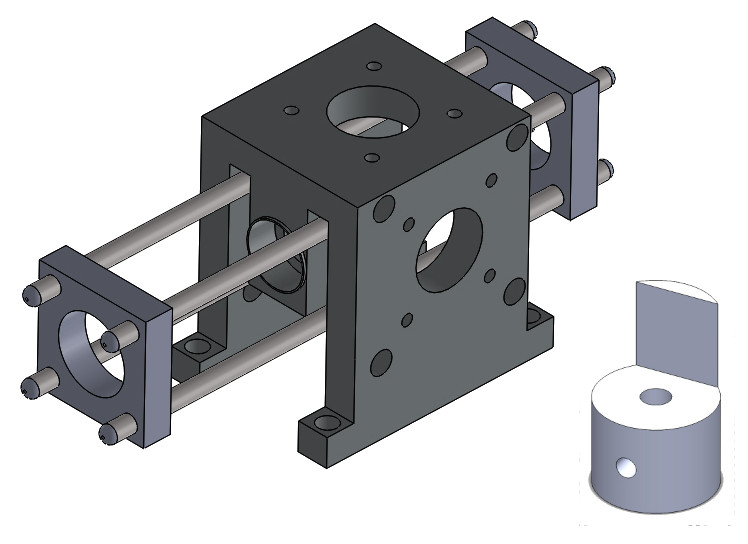
\includegraphics[width=\textwidth]{fig/perfilador/soporte_labo6}
                \label{fig:pieza}
                \end{figure}
            \end{column}
        \end{columns}
    \end{onlyenv}

    \begin{onlyenv}<3>
        Electrónica de adquisición
        \begin{columns}[c]
            \begin{column}{0.3\textwidth}
                \begin{figure}
                    \centering
                    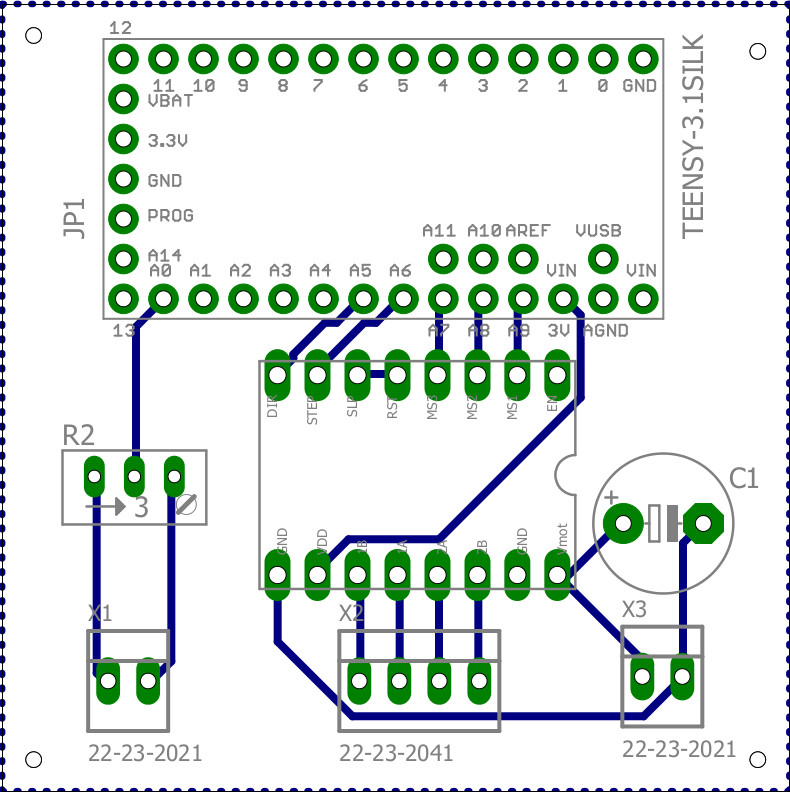
\includegraphics[width=\textwidth]{fig/circuito/circuito_labo6.jpg}
                    \label{fig:circuito}
                \end{figure}
            \end{column}
        %
            \begin{column}{0.6\textwidth}
                \begin{itemize}
                    \item uC Teensy v3.2. CPU 96MHz, y 64KiB RAM. ADC 1Msps max.
                    \item Pololu A4988. Motores hasta 1.5A por fase
                    \item Máxima adquisición de 24 perfiles por segundo, limitación del motor/uC/Software. 
                    \item Buffer de puerto serie de 1200 datos, se ajusta la medición
                    \item Software de ajuste en continuo cambio. Hecho en Python
                \end{itemize}
            \end{column}
        \end{columns}
    \end{onlyenv}
    
    \begin{onlyenv}<4>
        Mediciones de calibración
        \begin{columns}[c]
            \begin{column}{0.4\textwidth}
               \begin{itemize}
                    \item Medición a salida de colimador F220FC.
                    \item Diferencia apreciable de tamaño de haz entre transiciones. De origen mecánico
                    \item Fotodiodo saturado al usar resistencia de carga enorme (para amplificar).
                \end{itemize}
            \end{column}

            \begin{column}{0.6\textwidth}
                \begin{figure}
                    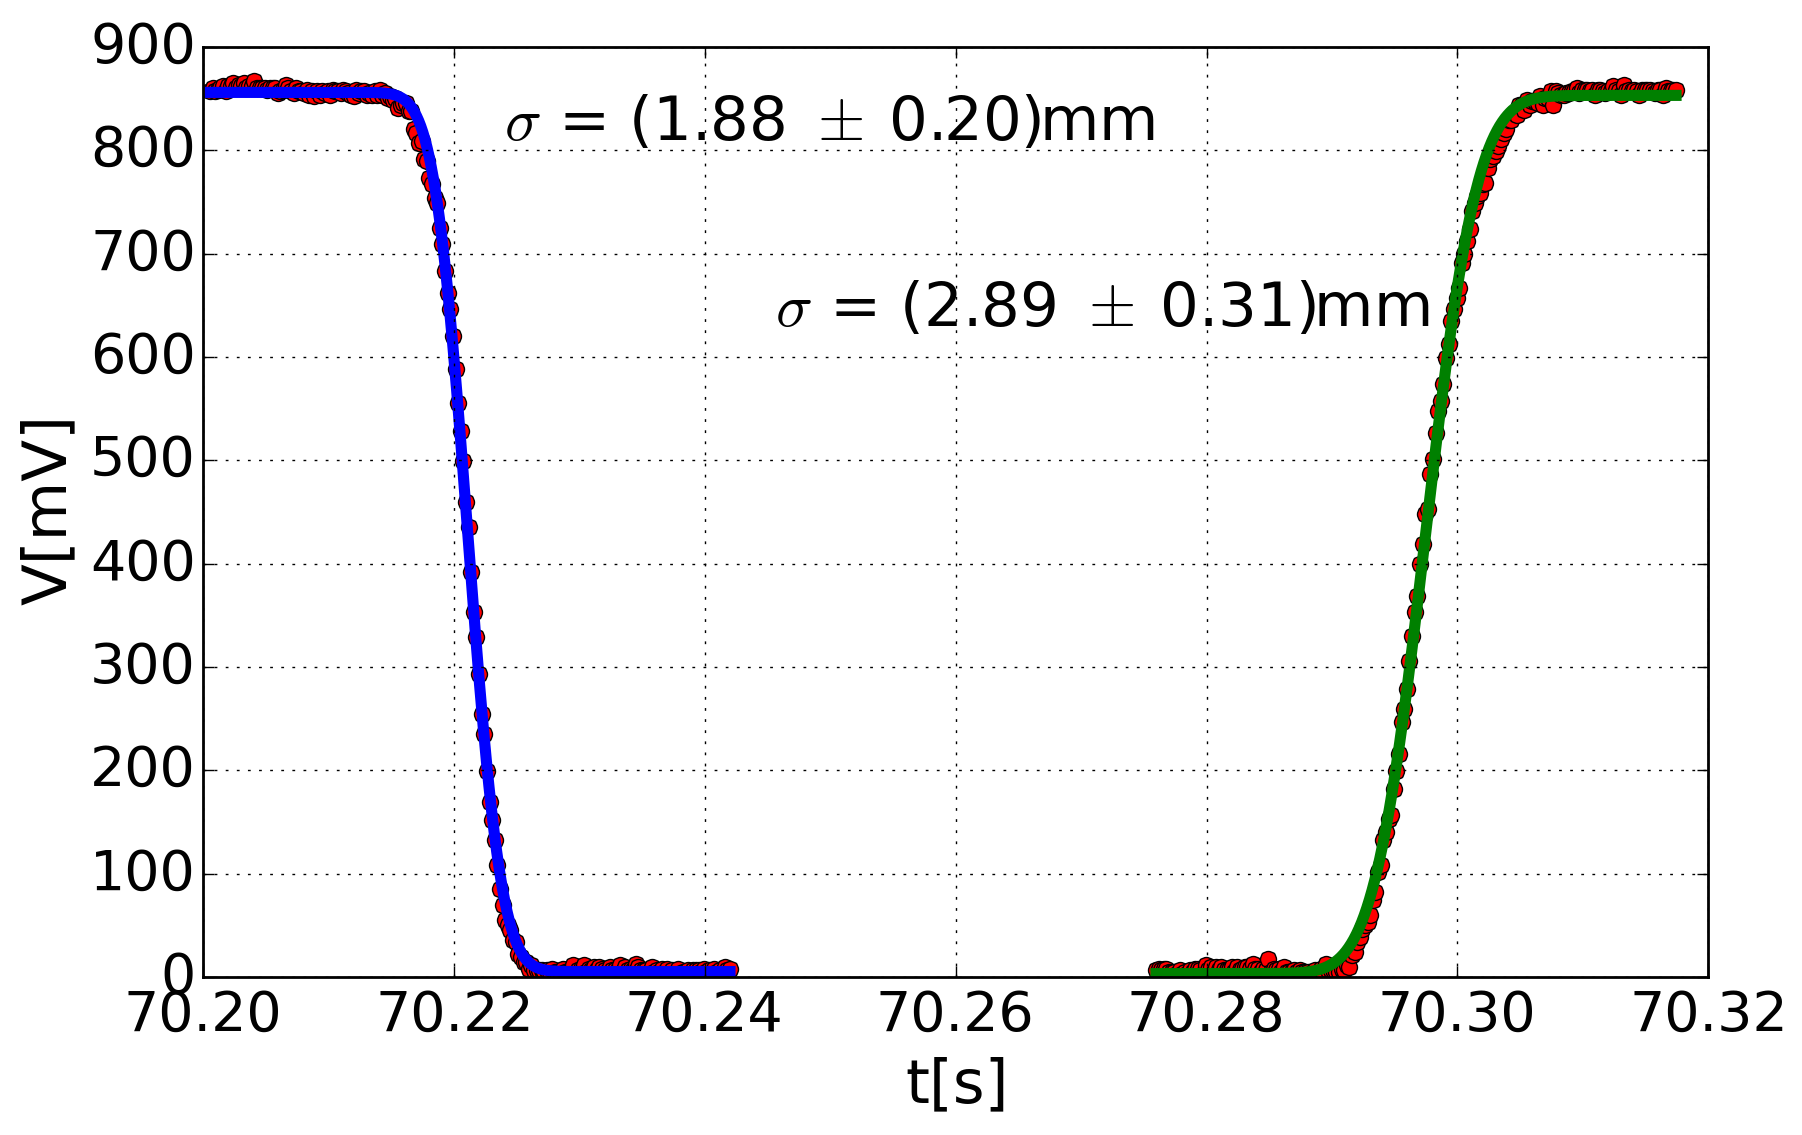
\includegraphics[width=\textwidth]{fig/perfilador/fit_data_labo6}
                    \label{fig:perfilador/fit_data_labo6}
                \end{figure} 
            \end{column}
        \end{columns}
        
    \end{onlyenv}
    
\end{frame}

%\begin{frame}{Objetivos en Laboratorio 7}
%\begin{itemize}
% \item Continuar el diseño del perfilador, adaptarlo a los diferentes setups del laboratorio y mejorarlo
% \item Construir un polarímetro con tecnología ya desarrollada para el perfilador
% \item Diseñar y construir un espectrómetro portátil a partir del IC Hamamatsu C12666MA
% \end{itemize}
%\end{frame}


\section{Mejoras de Labo 7}

\begin{frame}{Perfilador en Laboratorio 7}
    \begin{onlyenv}<1>
        
    
    Primera iteración mecánica
    \begin{columns}[c]
        \begin{column}{0.4\textwidth}
            \begin{itemize}
                \item Soporte adosable a la mesa óptica por perros. Facil colocación
                \item Motor encastrado en soporte. No hay artefactos mecánicos
                \item Tambor de metal con superficie no reflectante
                \item No permite medir fácilmente en el otro eje. Habrá otra iteración
            \end{itemize}
        \end{column}
        \begin{column}{0.5\textwidth}
            \begin{figure}
                \centering
                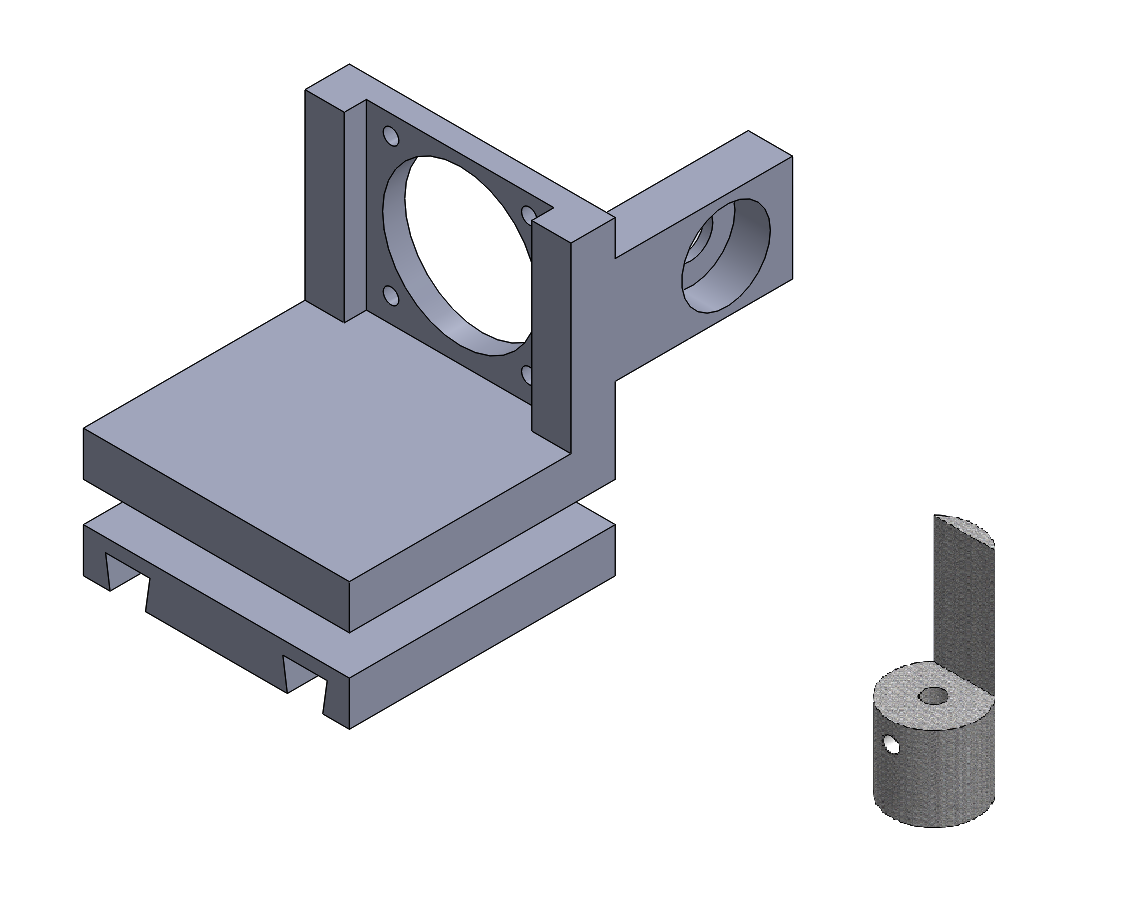
\includegraphics[width=\textwidth]{fig/perfilador/soporte_labo7_1}
             
                \label{fig:soporte_labo7}
            \end{figure}
        \end{column}
    \end{columns}
    \end{onlyenv}
    \begin{onlyenv}<2>
        
    Segunda iteración mecánica
    \begin{columns}[c]
        \begin{column}{0.4\textwidth}
            \begin{figure}
                \centering
                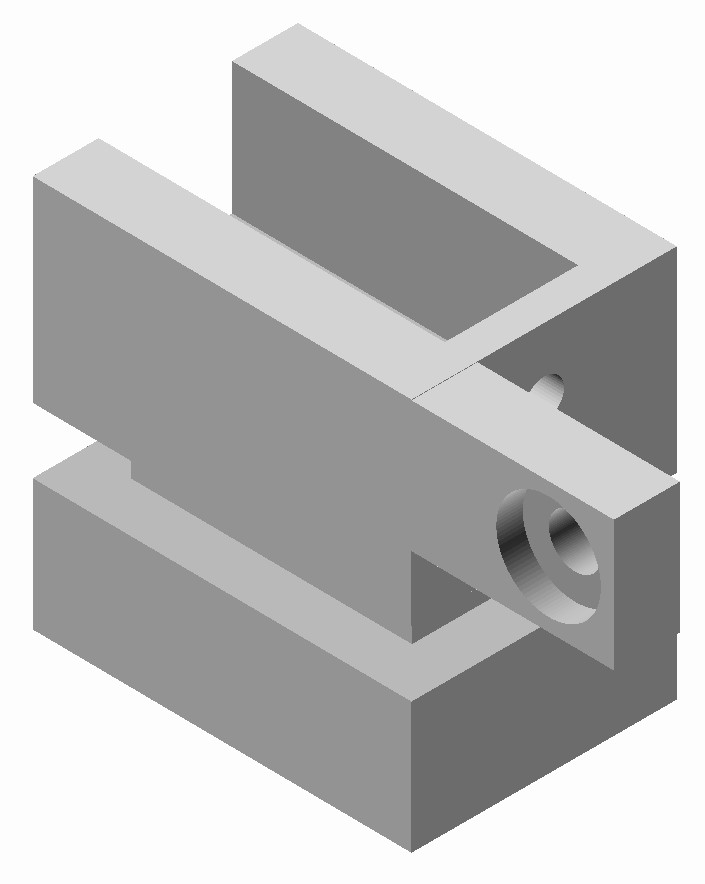
\includegraphics[width=\textwidth]{fig/perfilador/soporte_labo7_2}
             
                \label{fig:soporte_labo7}
            \end{figure}
        \end{column}
        \begin{column}{0.5\textwidth}
            \begin{itemize}
                \item  Motor NEMA 8, reduce un 500\% el tamaño.
                \item  Soporte fácil de colocar sobre la mesa óptica y sobre un soporte en altura
                \item  Tambor reimpreso en plástico
            \end{itemize}
            
        \end{column}
    \end{columns}
    \end{onlyenv}
\end{frame}



\begin{frame}{Electrónica de adquisición}
\begin{columns}[c]
    \begin{column}{0.5\textwidth}
        \begin{itemize}
        \item Considerado un amplificador de corriente. Se mide con amplificador de corriente Standford SR750 y se observa mejoras substanciales
        \item Implementado amplificador de transimpedancia con fotodiodo no polarizado. 
        \item Mejor respuesta en frecuencia y no satura el fotodiodo
        \end{itemize}
    \end{column}
    \begin{column}{0.4\textwidth}
        \begin{figure}[H]
        \centering
        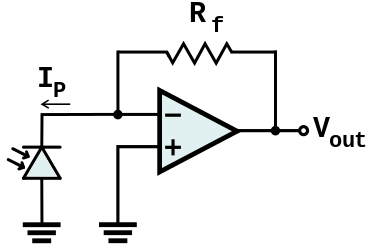
\includegraphics[width=1.1\textwidth]{fig/circuito/amp/TIA.png}
        \label{fig:circuito/amp/TIA}
        \end{figure}
    \end{column}
\end{columns}



\end{frame}

\begin{frame}{Calibración de amplificador}

\begin{columns}[c]
    \begin{column}{0.4\textwidth}
        \begin{itemize}
        \item Amplificador con LM358. Con fuente simple
        \item Respuesta al escalón de 0,4V$\,\mu$s$^{-1}$. 4 veces más grande de la necesaria
        \item Rango lineal bastnate amplio, pero no acusa corriente nula. Se puede buscar otro amplificador. Suficiente para la amplicación
        \end{itemize}
    \end{column}
    %
    \begin{column}{0.5\textwidth}
        \vspace{-1em}
        \begin{figure}[H]
            \centering
            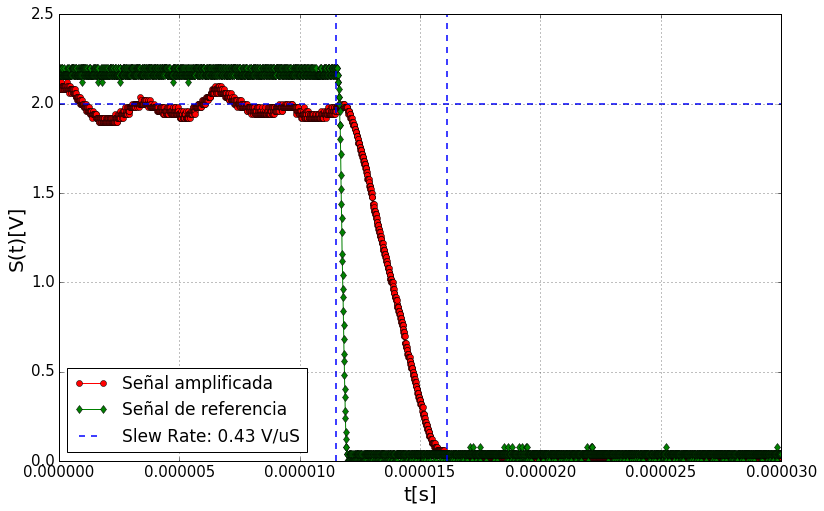
\includegraphics[width=\textwidth]{fig/circuito/amp/transicion_amp}
            \label{fig:transicion_amp}
        \end{figure}
        \vspace{-2em}
        \begin{figure}[H]
            \centering
            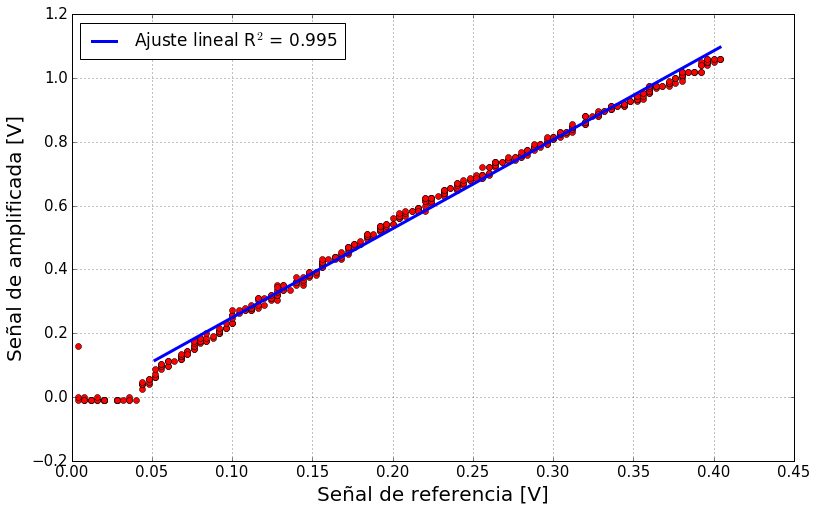
\includegraphics[width=\textwidth]{fig/circuito/amp/lin_amp}
            \label{fig:circuito/amp/lin_amp}
        \end{figure}
    \end{column}
\end{columns}

%La señales obtenidas con el fotodiodo polarizado en inversa y con una resistencia de carga son muy ruidosas. Se amplifica el ruido térmico, ruido de fuente y ruidos lumínico de fondo.
%Se procede a implementar un amplificador de transimpedancia: transforma corriente en tensión. El fotodiodo no se lo polariza, lo que permite mejor respuesta en frecuencia. 


\end{frame}

\begin{frame}{Generación de sensores portátiles}
\begin{onlyenv}<1>
    \begin{columns}[c]
        \begin{column}{.5\textwidth}
        Spark Photon
        \begin{itemize}
        \item ARM Cortex M3 120MHz con stack WiFi. \\Internet of the Things
        \item 128KiB RAM y 1MiB FLASH
        \item Programación en la nube, permite actualizaciones OTA.
        \item API de programación más poderosa. C++ por defecto
        \end{itemize}
        \end{column}

        \begin{column}{.3\textwidth}
            \begin{figure}
                \centering
                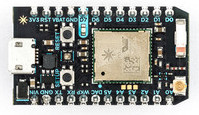
\includegraphics[width=\textwidth]{fig/circuito/photon}
                \label{fig:circuito/photon}
            \end{figure}
        \end{column}
    \end{columns}
\end{onlyenv}

\begin{onlyenv}<2>
    \begin{block}{Resultados con este uC}
        \begin{itemize}
            \item Se pudo mover el motor hasta 27,5RPS. \\PWM mejor implementado
            \item Conexión TCP permite mandar hasta de 2000 datos. Depende de la red WiFi
            \item Adquisición de datos cada 10$\mu$s o 100ksps. Más de lo necesario
        \end{itemize}
    \end{block}
\end{onlyenv}

\end{frame}

\begin{frame}{Software de adquisición}

\begin{itemize}
\item Programa efectuado enteramente Python.
\item Código libre para ser adaptado
\item Interfaz web, es portable y fácil de instalar
\item Permite obtener los datos crudos para hacer otros análisis.
\item Algoritmo de ajuste basado en técnicas de reconocimiento de imágenes
\end{itemize}



\end{frame}

\section{Mediciones}


\begin{frame}{Mediciones con el perfilador}

\begin{onlyenv}<1>
Salida de colimador F280FC del SPIM
\begin{columns}[t]
\begin{column}{0.5\textwidth}
    \begin{figure}[H]
    \centering
    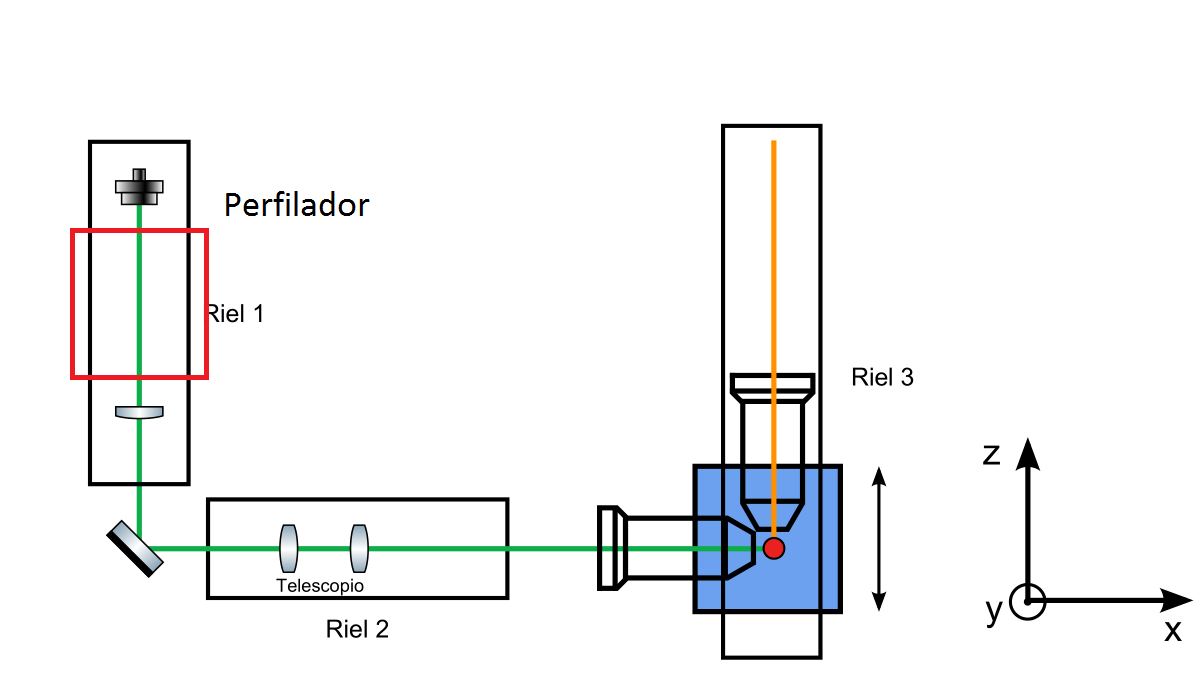
\includegraphics[width=\textwidth]{fig/perfilador/spim_riel_perfilador.png}
    \label{fig:spim_riel_perfilador}
    \end{figure}
\end{column}
%
    \begin{column}{0.5\textwidth}
        \vspace{-2em}
        \begin{figure}[H]
            \centering
            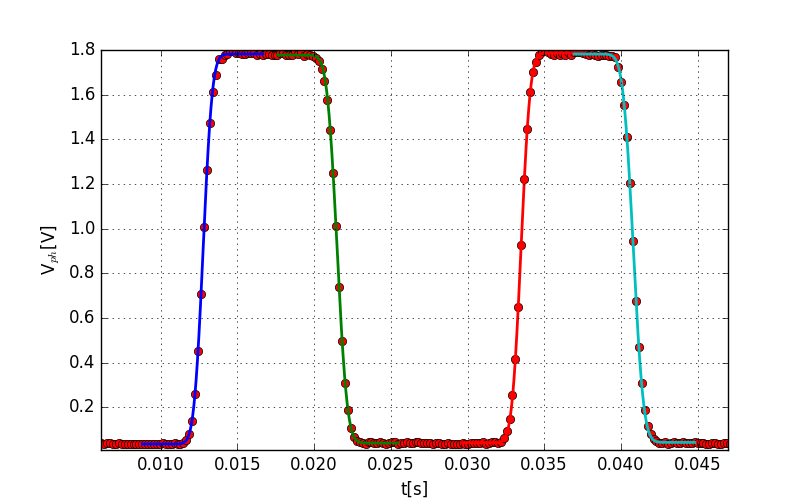
\includegraphics[width=\textwidth]{fig/perfilador/spim_foco_zoom.png}
            \label{fig:spim_foco_zoom}
        \end{figure}
        \vspace{-1em}
        
    
    \end{column}
    
\end{columns}

    \begin{itemize}
            \item Inicio del riel:\\ $\sigma = (3,03 \pm 0,15)\,\text{mm}$
            \item Fin del riel:\\ $\sigma = (3,02 \pm 0,18)\,\text{mm}$
    \end{itemize}
    Colimador \underline{efectivamente colima el haz}
\end{onlyenv}

%\begin{onlyenv}<2>

%Lightsheet del SPIM
%\begin{columns}[c]
%\begin{column}{0.5\textwidth}
%    \begin{figure}[H]
%        \centering
%        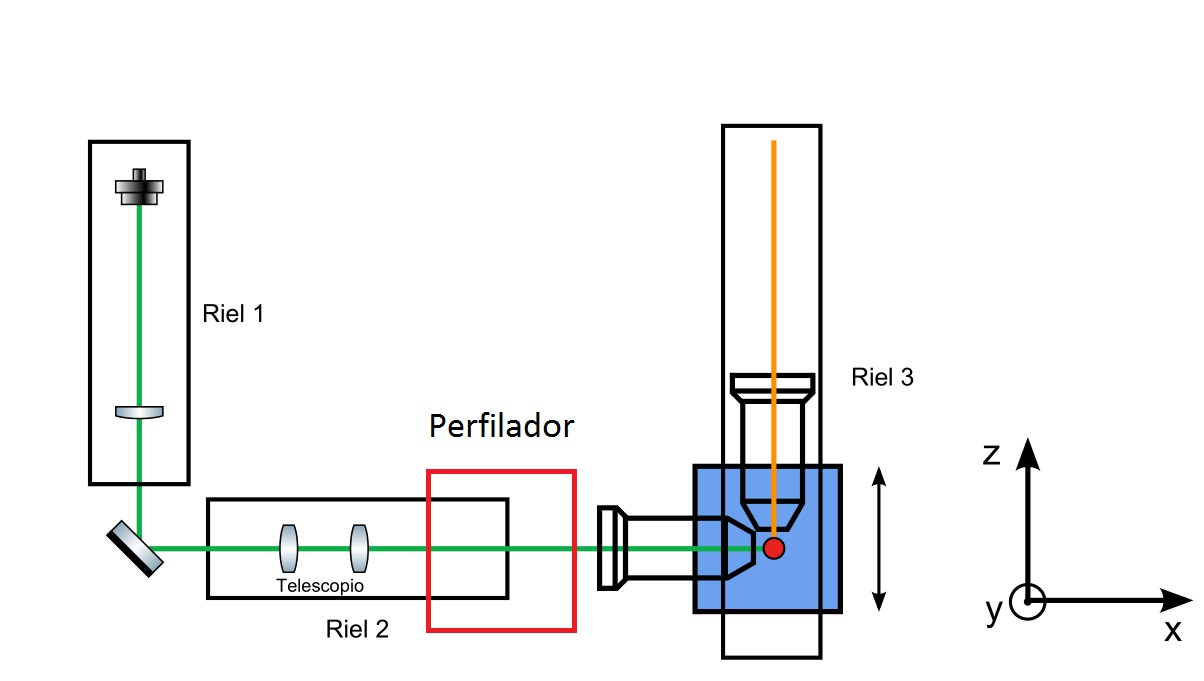
\includegraphics[width=\textwidth]{fig/spim_lightsheet_perfilador}
%        \label{fig:data_teensy}
%    \end{figure}
%\end{column}
%\begin{column}{0.5\textwidth}
%    \vspace{-3em}
%    \begin{figure}[H]
%        \centering
%        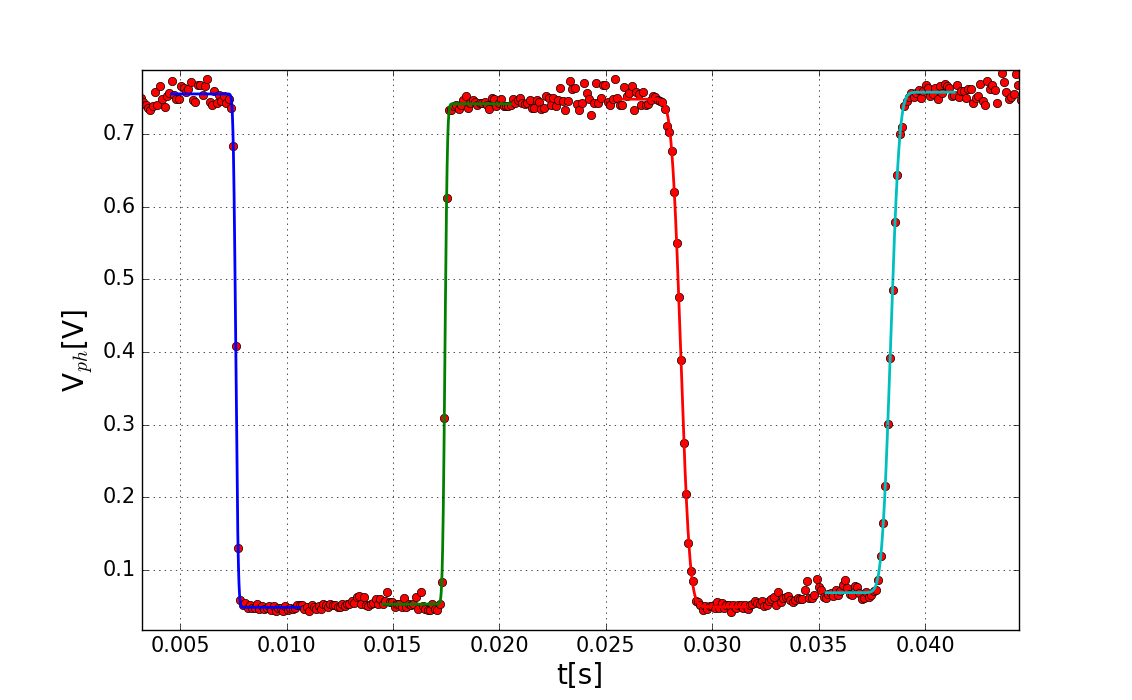
\includegraphics[width=\textwidth]{fig/spim_lightsheet}
%        \label{fig:data_teensy}
%    \end{figure}
%    \vspace{-1em}
%    Medición a \\d$\approx$80$\,$mm del fin del telescopio
%    $\sigma_1 = (0,55 \pm 0,02)\,\text{mm}$\\
%    $\sigma_2 = (2,11 \pm 0,05)\,\text{mm}$\\
%    \end{column}
%\end{columns}
%\vspace{1em}
%Las transiciones acusan una \underline{divergencia} apreciable.

%\end{onlyenv}


\begin{onlyenv}<3>
    \begin{block}{Conclusiones de esta medición}
        \begin{itemize}
            \item Se pudo caracterizar el haz dentro del SPIM en todo el trazado
            \item El perfilador fue capaz de medir la divergencia \underline{con solo un set de mediciones}.
            \item El tamaño de la cintura del haz es importante para el microscopio, y tenemos una medición directa fácil de efectuar
        \end{itemize}
    \end{block}
\end{onlyenv}

%\begin{onlyenv}<5>
%Láser Helio Neon 05-LGP-193. $d=80\text{mm}$
%\begin{minipage}[t]{0.5\textwidth}
%\begin{figure}[H]
%\centering
%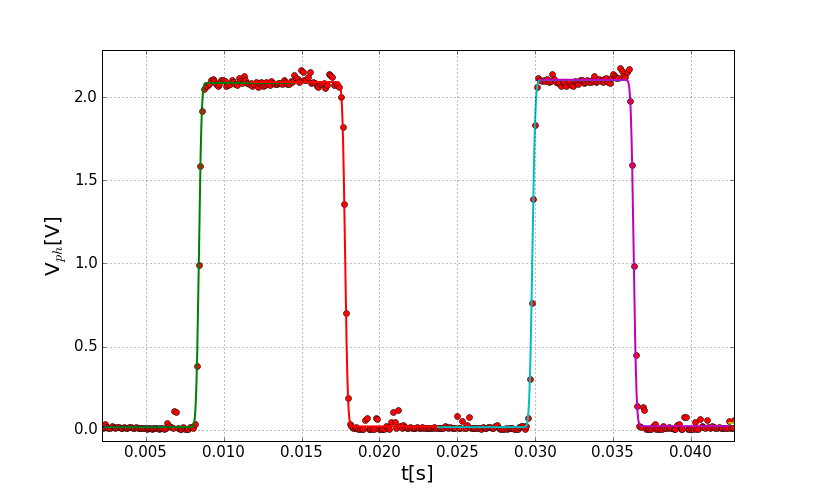
\includegraphics[width=\textwidth]{fig/he_ne_verde_zoom.png}
%\label{fig:data_teensy}
%\end{figure}
%\end{minipage}
%\begin{minipage}[t]{0.46\textwidth}
%\vspace{2em}
%$\sigma = (0,838 \pm 0,20)\,\text{mm}$\\
%Consistente con documentación.
%\end{minipage}
%\end{onlyenv}
\end{frame}





\begin{frame}[t,fragile]{Proyecto SOMA (Sistema de OptoMecánica Abierta)}

\centering

\begin{figure}[H]
\centering

\includegraphics[width=0.4\textwidth]{fig/proyecto_soma}
%\caption{}
\label{fig:soma}
\end{figure}

\begin{itemize}
\item Plataforma abierta de instrumental opto-mecánico
\item Diseño con énfasis en la reproducibilidad, con tecnología de impresora 3D o mecanizado automático.
\item Electrónica libre, controlada por software creado con tecnologías libres.
\end{itemize}

Página del proyecto: \url{http://lec.df.uba.ar/soma}

\end{frame}


%\begin{frame}{Lo que falta}

%\begin{itemize}
%\item Se espera que para fines de mayo esté disponible el espectrómetro. Adaptar el circuito para usar el espectrómetro.
%\item Alineación del SPIM para mejorar el lightsheet a la salida de la lente cilindrica.
%\item Construcción de un polarimetro automático portátil. 
%\item Construcción de un soporte mecánico y la adquisición de datos del espectrómetro.
%\end{itemize}


%\end{frame}



\begin{frame}[plain]{}
\centering

\Huge
Gracias

\end{frame}
